\documentclass[11pt]{article}

\usepackage{cite}
\usepackage{color}
\usepackage{graphicx}
\usepackage[hidelinks]{hyperref}
\usepackage{listings}
\usepackage{pdfpages}

\graphicspath{{../diagram}{../graphs}}


\author{Ogier Bouvier}
\date{\today}
\title{A zero-copy key-value store in Rust}

\begin{document}

\maketitle
\pagenumbering{gobble}
\tableofcontents
\newpage

\pagenumbering{arabic}
\setcounter{page}{1}
\section{Abstract}

The state of the art today for high-speed networking involves kernel
bypassing techniques making use of software such as DPDK to reduce the
overhead typically associated with kernel based networking. Such
software is usually much faster than traditional kernel networking,
mostly due to avoidance of context switches and data copies between
kernel and user space, especially when processing lots of small
packets which often happens in the case of key-value stores such as
memcached. Nonetheless these systems are far from perfect. First,
having all the  networking code and the user application inside the
same address space means that user code can corrupt the networking
stack very easily. Secondly, development of such applications is also
much more cumbersome than traditional kernel based approaches, indeed
having the user program in the same address space as the networking
code creates the need for it to be aware of low level networking
details that traditional applications don't need to worry about.The
necessity to handle this kind of networking details make kernel bypass
application much more time consuming and error-prone to develop than
regular socket based ones. Another problem these kind of systems
encounter is their inability to ensure safety, i.e.\ that data being
held in the networking stack is not modified by the user program
(which still holds a pointer to it) while for example waiting for a
TCP ACK.

\subsection{Rust}

We make the claim that Rust~\cite{rustbook} is a better suited
language than C for kernel bypass networked applications. The safety
guarantees Rust brings are very well suited for this kind of
applications, while the performance loss (if any) is negligible. As an
additional benefit Rust allows code to be much more concise and
abstract while drastically cutting down on the memory and concurrency
bug tracking time. Its memory management model will also prove
invaluable when ensuring integrity of data in between the networking
stack and the user application.

As a proof of concept we implement a key-value store on top of
DPDK in order to prove that it is doable as well as reasonable,
performance-wise, to use Rust in this kind of scenario.

\section{Rust}

Rust is a systems programming language from Mozilla Research, stemming
from Mozilla's dissatisfaction with C++. As of today several parts of
Firefox's rendering engine, Servo, have been rewritten in Rust after
the language was deemed mature enough to do so. Rust is engineered to
provide a lot of safety guarantees, notably memory and concurrency
safety through its type system thereby eliminating a lot of common
problems in systems programming.

The strong Rust guarantees also speed up development significantly by
eliminating whole categories of bugs. Most importantly, Rust's type system
eliminates use-after-free, double-free, invalid pointers, memory leaks
and data-races. Overall, the time writing code is increasing since the
compiler will often refuse straight out to compile code that
potentially violates its guarantees. The counter-part to this is that
the time spent debugging is very much reduced. This is particularly
useful when tracking down data race bugs which are notoriously hard to
diagnose. Those kind of bugs are usually found much later in the
development cycle and are usually quite hard to reproduce since they
depend on a certain scheduling of the execution.

\subsection{Memory safety}

One of the most important feature of Rust is its guarantee of memory
safety, providing both the speed of manual memory management and the
safety of garbage collected languages.

To provide this feature, Rust introduces a new concept called
lifetimes and makes raw pointers second class citizens. These raw
pointers (such as that of C) can't be dereferenced since the compiler
can't guarantee that they are valid. Pointers are hard to validate and
verify statically mostly because of pointer arithmetic. References, on
the other hand, are guaranteed to always point to a valid memory
location. Like the references in C++, references in Rust do not allow
pointer arithmetic, they can only be created from a variable, which
ensures that the referenced memory is valid.

Lifetimes are the central part of Rust's memory safety
guarantees. They work in conjunction with references to ensure
that references are used correctly (i.e.\ not after the value they
refer to has been destroyed), since they allow the compiler to tell
when a reference might outlive the value it refers to. The combination
of lifetimes and references thus eliminate the dangling pointers
problem entirely. Lifetimes are Rust's way of eliminating the need for
garbage collection while not requiring users to manually manage
memory. A lifetime gets attached to each variable created, the
compiler then analyzes the control flow of the program to ensure that
references or values derived from that first value (such as reference
to a struct member) are not used after the value is destroyed.

However Rust is a at the core a systems programming language so we
need some way to bypass the safety restrictions it provides. This is
where the \textbf{unsafe}~\cite{rustonomicon} keyword comes in. This
keyword provides a way to tell the Rust compiler that a piece of code
upholds the memory safety guarantees even though the former can't
verify it statically. Handling of raw pointers and call to foreign
functions are cases where the use of \textbf{unsafe} is
required. Indeed other languages do not provide any of Rust's
guarantees and do not know about lifetimes. This problem also occurs
when developing kernels~\cite{redox}.
% ref to rust Kernel design paper and Rustonomicon
% also ref to redox?

\subsection{Concurrency safety}

Rust's type system also provides protection against data-races, a
common problem when using C usually solved through atomic operations
and locks. While it is possible to solve this kind of problems in C,
it requires careful design and is an error-prone task. Rust therefore
allows quicker and safer development of concurrent software. This safety
does not come for free though. In order to guarantee that there is no
data-race anywhere, Rust only allows either one mutable reference or
any number of immutable reference to any given variable. By doing
that, the compiler can ensure that the variable will only be read
concurrently or written exclusively.

Even though we speak of concurrency safety, Rust does not provide
protection against deadlocks. This is a far too complex task for
static analysis in a compiler since it requires graph analysis calls
and sometimes produces false positives.
% cite http://groups.csail.mit.edu/commit/papers/05/williams-ecoop05-slides.pdf

However, the Rust standard library provides safe ways to mutate shared
variables. As an example the RwLock standard library structure allows
creating mutable reference to a value from an immutable RwLock instance.

\subsection{Performance}

Being a systems programming language, performance is critical to
Rust. All the aforementioned guarantees are enforced statically so
they do not incur any performance penalty. Removing pointer aliasing
from the language also allows the compiler to do many optimizations
that are not feasible safely in C or C++. As to the performance of the
generated assembly code, Rust utilizes the LLVM compiler
infrastructure and thus benefits from all the work that was done
there. Rust also features what the Rust developers call 0-cost
abstraction. Idiomatic Rust makes heavy use of closures, and that
would incur, in some languages, a slight degradation of
performance. But, in Rust, closure can be, most of the time, inlined
thus making as if the programmer wrote the concrete code while
allowing the interface to remain abstract.

In this regard, Rust combines the best of both worlds, high-level
readable and abstract code while also having performance close to that
of other systems programming languages.

\section{Design}

\subsection{Goals} \label{design-goals}

In order to be truly high-performance, the store should ideally
support fast, lock-free and zero-copy insertion and retrieval. That
means we need to come up with a concurrency control scheme to support
concurrent lock-free updates. Since we don't need to provide strong
consistency guarantees (other than being eventually consistent), we
can rely on an optimistic multi version concurrency control scheme for
simplicity of implementation and speed.

We should also provide an efficient and convenient interface to the
network. This interface should also uphold the zero copy property that
is provided by the store in order to provide a true zero copy
key-value store. If we succeed in providing such an interface, further
development of high-performance networking applications in Rust would
be much simpler.

\subsection{Local store} \label{design-overview}

The first step in providing an efficient key-value store is to
have an efficient hashmap to store and retrieve key value pairs
rapidly once the request have been parsed. This also poses the
additional challenge of working within the limit of Rust's borrow
checker and smart use of unsafe. Care was also taken to ensure that
the resulting hashmap is suitable for zero-copy insertion and
retrieval. This means that the ownership of values inside the hashmap
has to be carefully managed to ensure client can retrieve and use
values from the hashmap concurrently with the hashmap being modified.

We go with the following design. The top level table is a contiguous
array of atomic pointers to overflow buckets. And in turn each
overflow bucket is a pointer to a key-value pair structure allowing
easy extraction of both keys and values, as shown in
\hyperref[fig:hashmap]{figure~\ref*{fig:hashmap}}.

\begin{figure}[htb!]
  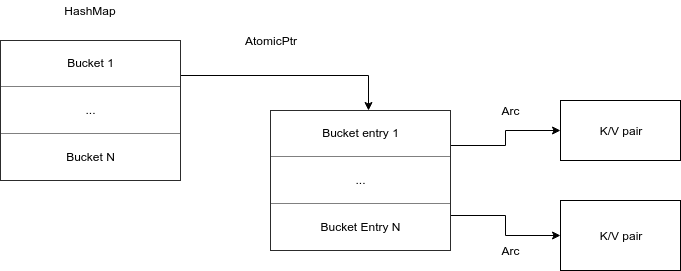
\includegraphics[width=\textwidth]{../diagram/amap1}
  \caption{Hashmap overview}
  \label{fig:hashmap}
\end{figure}

The pointers inside each overflow buckets are atomically reference
counted for multiple reasons. The first obvious one is that values
live for an undetermined amount of time and are shared between
multiple threads. The second reason is that the pointer to the data
does will not only reside in the hashmap itself but also in the
networking stack while waiting for an ACK, as shown in
\ref{fig:omvcc}.

\begin{figure}[htb!]
  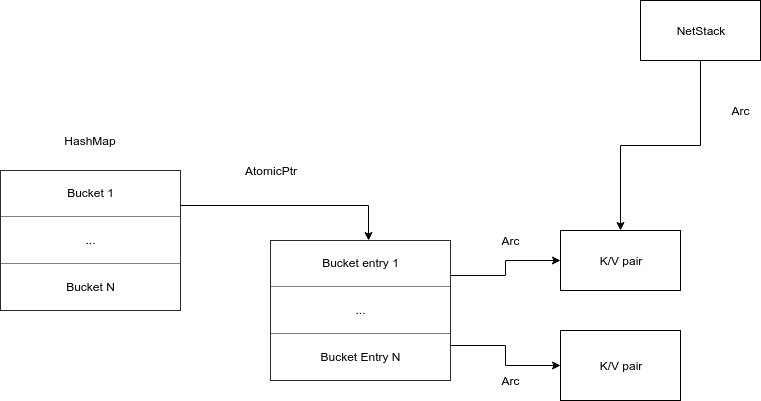
\includegraphics[width=\textwidth]{../diagram/cc1}
  \caption{Optimistic multi-version concurrency control}
  \label{fig:omvcc}
\end{figure}

Let's now see how we are going to perform updates in the store.

\begin{figure}[htb!]
  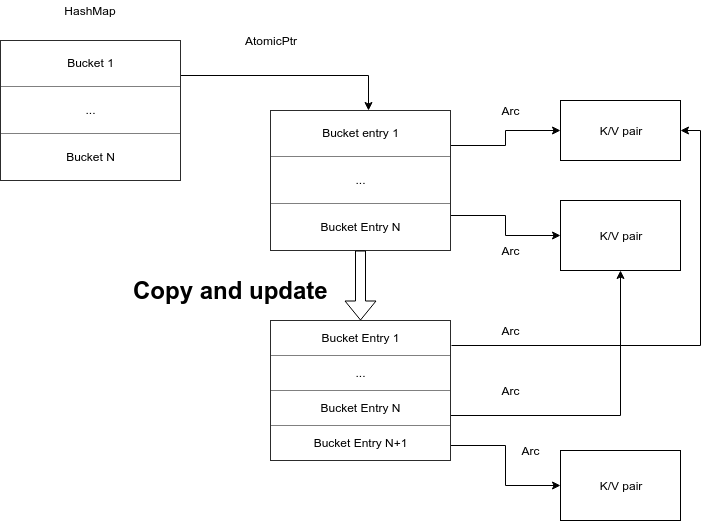
\includegraphics[width=\textwidth]{../diagram/amap2}
  \caption{Value insertion}
  \label{fig:omvcc-insert}
\end{figure}

We first copy the entire overflow bucket, as shown in
~\ref{fig:omvcc-insert}. Since the overflow bucket is only made out of
pointers this is not a costly operation. We also take care to increase
the reference count of each pointer in the overflow bucket to avoid
early frees of the values. Once we have our copy we build the new
version of the overflow bucket locally. Once we have built the new
version we attempt to swap it atomically inside the top-level
table, ~\ref{fig:omvcc-swap}. If the compare and swap fails, we simply
retry by fetching the new value and constructing our own once
again. In the case where the swap is successful, the now-old value of
the bucket may be in use by some concurrent read or write operation,
we thus can't free it right away. This is where the choice of
atomically reference counted pointers comes in handy. We just have to
decrease the reference count of the old bucket, freeing it if we had
the last reference to it.

\begin{figure}
  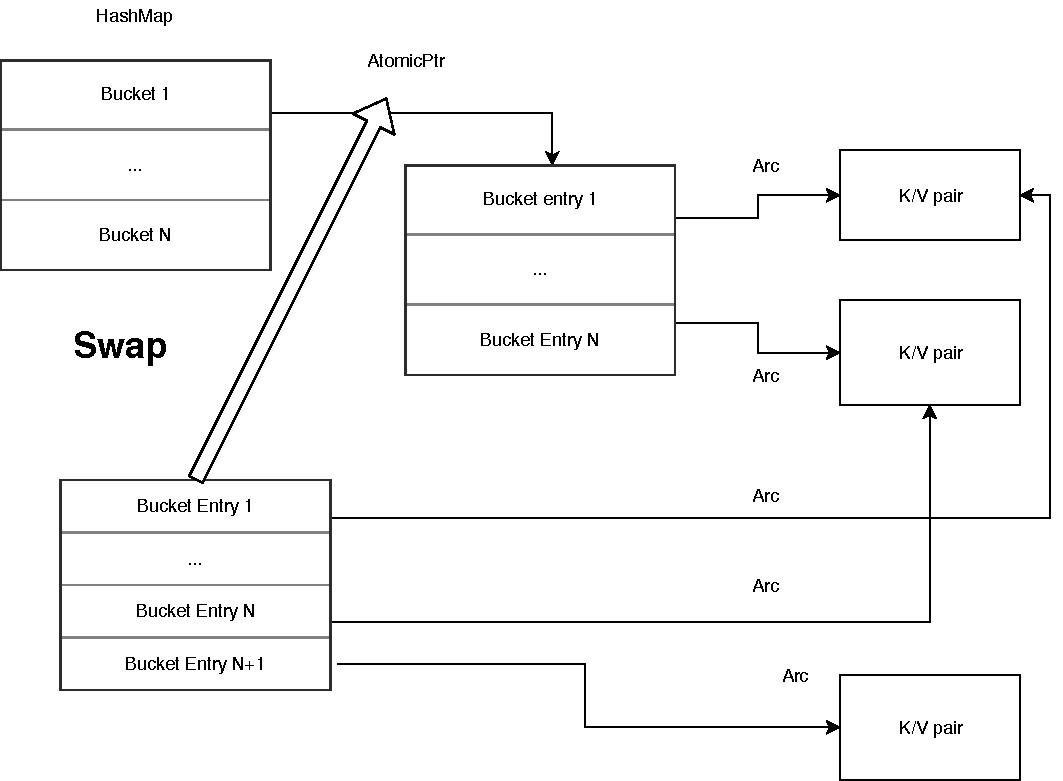
\includegraphics[width=\textwidth]{../diagram/amap3}
  \caption{Bucket swapping}
  \label{fig:omvcc-swap}
\end{figure}

This lock-free design allows a fast and zero-copy insertion of values
inside the hashmap. The most expensive operation for an insert is
actually the atomic compare and swap. This can become a problem if
there is a lot of threads competing for the same bucket concurrently
since atomic operations can cause stalling. However this would be a
problem only if the workload we are serving is a skewed write-heavy
workload. Since a typical workload on key-value stores implies a
majority of reads compared to writes (the Facebook USR load is only
0.2\% writes), this won't be a problem in our target use case.

The case shown in ~\ref{fig:omvcc} actually showcases how we handle
data shared between the user program and the networking stack. Since
we aim to provide a reliable networking protocol, at some point the
data will be passed to the networking stack for transmission. At this
point the networking stack will hold on to the data until it is
acknowledged by the other end. Our design even allows values to be
removed from the hashmap while still being held in the networking
stack for retransmission, see~\ref{fig:cc2}. The data is then only
referenced in the networking stack, and freed once it is successfully
acknowledged.

\begin{figure}[htb!]
  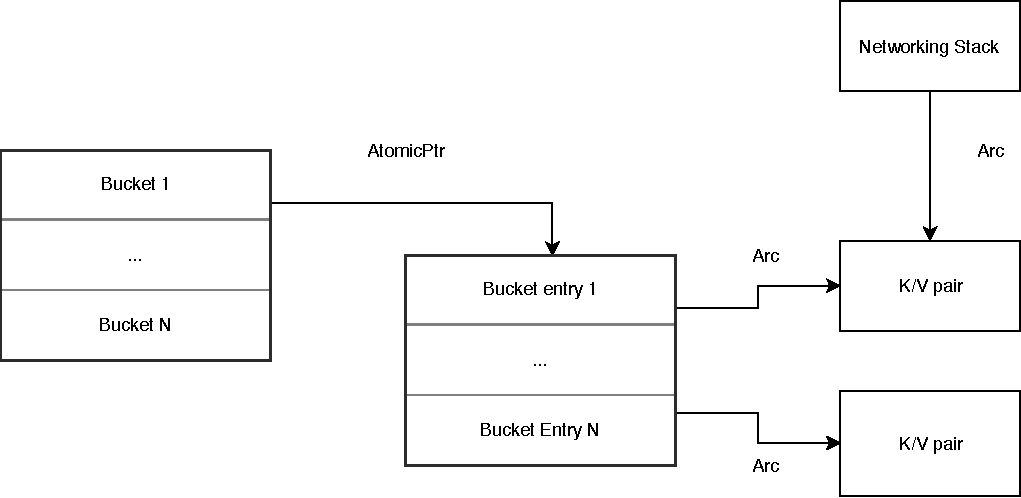
\includegraphics[width=\textwidth]{../diagram/cc2}
  \caption{Concurrent value removal}
  \label{fig:cc2}
\end{figure}

On another note, Rust's concurrency guarantees ensure that data held
in the networking stack can't be modified (since the networking stack
holds an immutable reference to it, there can't be any mutable
reference to that data). The problem of the user program still having
the pointer to the data thus becomes a non-problem since the compiler
ensures that the user program does not modify it.

\subsection{UDP stack}

One thing we need to consider also is the type of values that are
gonna be stored in the hashmap. Indeed, the key and values of the
hashmap are, in the end, going to be coming from the network. The
actual key-value datastructure used is thus critically important,
since it will be the interface for manipulating packet data in a
zero-copy fashion.

Since we will be in a run to completion execution model the standard
socket API calls (recv and send) is not a possible API\@. We thus have
a callback oriented UDP stack. When the user application creates a
new socket on the stack, a callback is provided. This callback is then
used when the networking stack receives a packet.

\subsection{R2P2 interface}

R2P2, the Request Response Pair Protocol, is a recent RPC protocol
from EPFL's Datacenter Systems Laboratory. To allow for rapid testing
and benchmarking, the choice was made to use R2P2 as an RPC protocol
for our key value store.

We provide an R2P2 interface for client interfacing. This R2P2 stack
is the interface between the user application itself (the key-value
store in our case) and the UDP networking stack and handles request
parsing, response sending and retransmissions when needed.

As is typical in RTC packet processing models, tie-in to the user
application will be handled through the use of callbacks. The user
application registers its `RequestCallback' when initializing the R2P2
stack.

The stack then listens on incoming UDP packets, processing them as
required. Packets are grouped request-wise into a HashMap while
waiting for all packets in the request to be received. Once the
request is complete the user registered callback is called on the
complete request to produce a matching response. That response is then
stored for potential retransmission while awaiting acknowledgement
from the remote host.

\section{Implementation}

We now discuss how our abstract design translates into a concrete Rust
implementation, including how it ties into the Rust standard library
and what are the individual components of each part of the system.

\subsection{AtomicBox}

Unfortunately the rust standard library only provides a mean to
atomically swap raw pointers using the \textbf{AtomicPtr}
construct. This effectively forces us to make use of raw pointers,
thus not benefiting from any of Rust's memory safety guarantee and
potentially leading to memory corruption or leaks.

This leads to the \textbf{AtomicBox} abstraction, a safe wrapper
around \textbf{AtomicPtr}, that we use to build our OMVCC hashmap.
The AtomicBox makes use of X86 CAS instructions to improve on Arc.
Arc provides an atomic reference count and AtomicBox provides an
atomic reference count as well the possibility to atomically swap that
value. Since every value is atomically reference counted it will stay
allocated as long as any reference to it still exists while allowing
new requests to fetch the newer value to do their work. Updates are
made using the value atomically fetched at that point in time,
creating a copy, modifying it as appropriate and then swapping it back
with the old one. If the swap succeeds the old value's reference count
is decreased (and dropped if we had the last reference), effectively
providing an optimistic multi-version concurrency control. If the swap
fails, i.e\. someone already swapped it with another value, we repeat
the same process until the swap is successful.

\subsection{Concurrency control}

To build the AtomicBox abstraction we make use of the capability of
Arc to be transformed into raw pointers, thus allowing a user to
control exactly how long the memory on the heap lives. The reference
can then be transformed back into an Arc, though since we make use of
raw pointers this requires using \textbf{unsafe}.

This means our AtomicBox abstraction also handles atomic reference
counting of the values it contains. Meaning that the values live as
long as there exists a reference to them anywhere. We thus have an
optimistic multi-version concurrency control scheme. A concurrent GET
and PUT therefore do not interfere with each other since the GET will
fetch a version of the bucket while the PUT will create a new one that
is then swapped independently from the one accessed by the GET
request.

\subsection{Memory management}

Since they are to be shared amongst threads, all the hashmap
components are allocated on the heap. As they are  all in the same
size range (most of them consists only of one or two pointers), we
make the claim that memory fragmentation is not gonna be an issue in
our case. Indeed most of the heavy allocation are coming from DPDK
allocating memory buffers from Linux's \textbf{hugepages} and thus
won't affect the heap.

\subsection{UDP}

We also aim to provide an efficient easy to use UDP stack on top of
NetBricks to facilitate development of other applications. This UDP
stack should use callbacks to hand over packets to the user program.

\section{Networking}

In this section we will delve in the networking part of the key-value
store, highlighting the Rust-DPDK interfacing as well as the different
APIs that we provide on top of said interface and how they
interconnect to form the final key-value store. We will also talk
about the challenges of providing a true zero-copy networking stack in
Rust on top of DPDK.

\subsection{Design overview}

Let's start with an overview of the system as a whole before diving
into the details of each individual piece.

\begin{figure}
  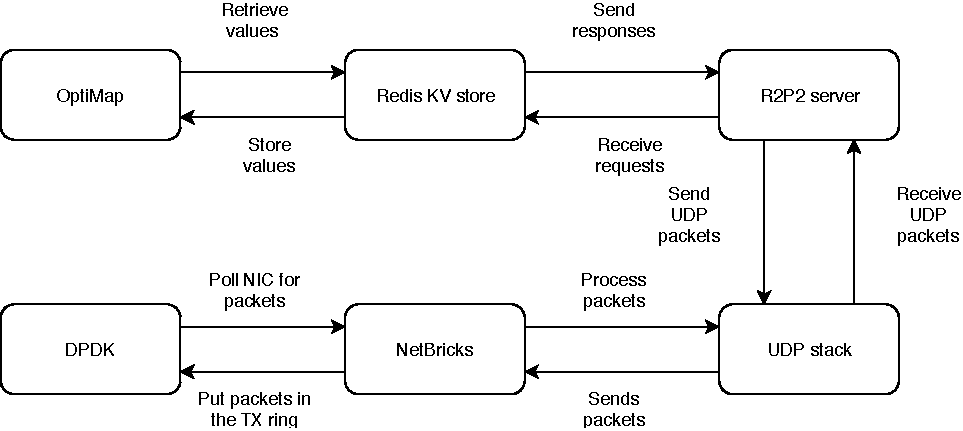
\includegraphics[width=\textwidth]{../diagram/overview}
  \caption{System overview}
  \label{fig:design-overview}
\end{figure}

Each packet is first received by DPDK from the NIC. The packets are
then processed through the NetBricks pipeline to be handed over to the
UDP stack. The UDP stack then filters and matches packets to a given
socket. Each socket has an associated callback registered by the
user. In our case, the socket are created by the R2P2 server which
uses them to receive R2P2 requests from the network. Once every packet
in a request has been received, the R2P2 server then invokes its own
user callback, this time called the Request Callback. This callback
is registered by the last layer in the system, the actual key-value
store. The key-value store uses R2P2 to satisfy requests in the Redis
protocol. This is also where our hashmap comes in (though it is used
all across the system), to store the key value pairs.

Let's now dive into more gory details about each part individually.

% TODO: diagram of how each piece is tied together

\subsection{DPDK}

As you probably know, DPDK is a kernel-bypass networking framework
developed by Intel, typically used for high-performance networking
applications. To support true zero-copy we are required to use some
form of kernel bypassing since the kernel networking is absolutely
not zero-copy. We thus implement all our networking on top of DPDK.

It is worth mentioning the Linux kernel socket flag for zero copy.
Though it does not provide guaranteed zero copy sending/receiving a
port of nginx using it saw a 9\% increase in performance with minimal
code changes. We chose not to use it though, since it would eliminate
one of the most interesting aspect of the project, the ability to have
a safe userspace networking stack in the same address space as the
user program.
% insert ref to paper

Since DPDK is written in C, we must first find some (ideally,
convenient) bindings allowing us to make calls into DPDK from Rust
code. One more thing to consider is the inherent unsafety in calling C
code from Rust. Since C code has none of the guarantees of Rust calls
to C functions must be in an unsafe block. A convenient safe Rust
interface is therefore a must for speed and ease of development.

\subsection{NetBricks}
NetBricks~\cite{netbricks} is a Rust framework on top of DPDK,
providing a clean and Rust-friendly API, as well as advanced packet
processing facilities. It is, though, aimed at rapid development of
network functions which does not quite fit our current target. A fork
was therefore necessary to modify it to suit the particular needs of a
host networking framework.

The fork comes with a few modifications to the NetBricks
framework. The first one is the inability of packets to cross thread
boundaries. Indeed since NetBricks is geared towards network functions
the packets are only meant to be processed by the user defined
pipeline and is deallocated after it has gone through the whole
pipeline. To remedy this we create the CrossPacket abstraction which
can be created from the standard NetBricks Packet and is able to cross
thread boundaries by being immutable. But we still need to be able to
send packets through NetBricks and NetBricks does not know how to
handle CrossPackets. It is therefore possible to convert a CrossPacket
to a Packet as well as the reverse.

The CrossPacket abstraction only contains a single immutable raw
pointers to a DPDK mbuf. This means that CrossPackets can be shared
across threads without the Rust compiler getting in the way. However
since the pointer to the mbuf is immutable this poses a problem when
sending the packet. Indeed DPDK stores headers in the same buffer as
the payload, meaning we can't easily send the same payload
concurrently to two different destination. The way to solve this is
make use of DPDK's mbuf chaining, the first mbuf in the chain being
local to the current thread (therefore being mutable) and the second
one being the immutable payload shared between threads. This is the
second notable modification we make to our NetBricks fork, the ability
to chain mbufs to maintain the immutability of the packets we received
from the network while maintaining the ability to send them
concurrently to different destinations.

One more thing that needs to be implemented in NetBricks is packets
living longer than the packet processing pipeline. Since NetBricks is
aimed at network function once a packet has gone through the packet
processing pipeline it has no reason to stay allocated (as in the case
of a firewall, when the decision has been made to forward the packet
it's not needed anymore). But in our case packets are longer lived, we
need to keep them in the store to answer queries later on. We then
need a way to prevent deallocation of packets once they leave the
pipeline. We make use of mbuf reference counts to do this. In our
segmented packets the headers always have a reference count of one,
indeed they are not needed once the packet has been sent successfully,
thus we let DPDK free them once the packet have gone through the
NIC. The payload on the other hand should not be deallocated after
sending, so we set its reference count to 2, thereby preventing DPDK
from freeing it. But we still need to free them once they are not
needed anymore. The problem here is that mbuf reference counts are not
atomic, this is a problem in our case since the same payload could be
sent from two different threads which will both need to increment
it. That means we need to wrap the actual payload and provide an
atomic reference counting capability.

\subsection{UDP stack}
The first step in the development of the key value store is obviously
to have some networking support. The choice of UDP makes sense in term
of ease and speed of development given the time constraints of the
project. Moreover, as we will see later on, the use of R2P2 (which
uses UDP as a transport protocol) as an RPC protocol makes a
working UDP stack a requirement.

The UDP stack ties in to NetBricks by registering a pipeline on all
available cores and using this pipeline to dispatch packets to the
correct socket. Each socket is stored in a hashmap in the stack by its
port. Upon receiving a packet the stack filters in multiple steps the
packets dropping invalid ones and routing the others to the correct
socket. The corresponding callback is then called on the packets one
by one.

The sending part of the networking stack uses a round-robin approach
and selects a different queue for each batch of packets. A more
sophisticated approach could be envisaged to avoid flooding a specific
port queue.

\subsection{R2P2 server}

We use a variant of the R2P2 protocol that adds active acknowledgement
from clients in order to reduce latency when packets are dropped. For
the sake of simplicity we also do not handle packets that are
delivered out of order, mostly to avoid resizing buffers used to store
the request while it is not completely received.

The R2P2 stack is built on top of the aforementioned UDP stack. The
R2P2 server registers a packet callback and then dispatches the packet
to the correct request after parsing the headers. Again the R2P2
server uses callbacks registered by the user application to handle
requests. These callbacks return a R2P2Response structure that is then
sent by the R2P2 server through the UDP stack.

The R2P2 server handles reliable delivery through client
acknowledgement. The response returned by the user callback is stored
in the R2P2 server while waiting for the acknowledgement and
retransmitted if need be.

\subsection{Key value store}

The key-value store uses a simplified version of the Redis
protocol. It only supports SET and GET requests, since the test
workload has no other type of requests.

The Redis server implementation interfaces with the R2P2 server through
the request callback registration mechanism. It then handles
construction of the actual value that will be stored in the
hashmap. The requirements for the actual hashmap value and key
datastructures are mostly to play nice with the Rust memory management
model and DPDK mbufs. Indeed since we use segmented packets, we need
the headers to be freed once the request has been satisfied but the
payload itself must be kept as long as either the hashmap or the
networking hold it. As the payload can be sent concurrently from
different threads we need some sort of atomic reference counting on
the mbufs. The problem here is that mbufs reference counts are not
atomic (they're plain 16 bits integer).

This leads us to the \textbf{Payload} abstraction. This structure combines a
convenient access to the value and key, but also the mbufs containing
that value and key. Since the structure contains the packet
themselves the Rust compiler ensures that access to the key and value
is bound to the lifetime of the packets actually containing them.

\section{Evaluation}

We now discuss the performance of our key-value against the USR
Facebook workload.

TODO: describe test machines

\subsection{Local store}

We first evaluate how the local hashmap performance, especially when
under a lot of load. We use UTF-8 string keys of 128 bytes with values
of 64 bits to simulate only copying pointers to packets from the
network. We generate a random workload for each of the 15 concurrent
thread and start them simultaneously. Each thread performs one million
GET and 1 million PUT request, on a previously initialized map.

\subsubsection{No collisions}

We first establish the optimal performance we can expect from the
hashmap by reducing the contention on the bucket, thus reducing the
amount of wasted work by threads trying to swap out the buckets
unsuccessfully. To this end, we allocate four times more buckets than
they are keys and using a uniform distribution when generating
workload. The set of keys is pre-determined and no new keys are
inserted throughout the test, meaning the size of each bucket will
stay constant.

\subsubsection{Artificial collision}

We now consider the case of a skewed and/or write heavy workload and
evaluate the performance of the hashmap in this scenario. In order to
simulate this, we reduce the number of buckets in the hashmap. This
artificial collision indeed introduces contention between threads for
buckets and will cause wasted work when two threads update the same
bucket concurrently.

\subsection{Networked store}

TODO once the R2P2 stack is working

\section{Conclusion}

We hope to have provided an easy to use and clear API to build upon
our system. We also think that we have proved that Rust is a valid
language to build kernel bypass networking in.

\subsection{Further work}

We finish by mentioning what features are missing or could be useful
in such a piece of software. We have provided a UDP stack on top of
NetBricks, even though in real-life scenario of networking
applications UDP is rarely used. A TCP stack on top of NetBricks would
therefore be a considerable improvement.

One other thing that makes sense to have is an ARP handler. In our
case we respond to a request, so we have both the source and
destination MAC addresses at hand. But in the case where we want to
send a packet to an arbitrary IP we need to figure out the destination
MAC address. This is where an ARP protocol handler would come in
handy.

With an ARP and TCP stack we would be close to a full featured
networking framework in Rust for kernel bypass. Such a system would
provide both the speed and the convenience of traditional socket based
networking while also providing better networking performance and the
safety of the Rust programming language.

\newpage
\pagenumbering{gobble}
\bibliographystyle{plain}
\bibliography{master}{}

\end{document}
%%% Local Variables:
%%% mode: latex
%%% TeX-master: t
%%% End:
